\section{Benchmarks}

\hidenum
\begin{frame}[noframenumbering]
\frametitle{Contents}
 \tableofcontents[currentsection,hideallsubsections]
\end{frame}
\shownum



\subsection{Benchmarks}

\begin{frame}
  \begin{block}{Non-Optimal Choices Throughout}
    \begin{enumerate}[<+-|alert@+>]
      \item Only free software used (no MKL, ACML, etc.)
      \item 1 core = 1 MPI process
      \item No tuning for data distribution, just the defaults
    \end{enumerate}
  \end{block}
\end{frame}

\begin{frame}
  \begin{block}{Benchmark Data}
    \begin{enumerate}[<+-|alert@+>]
      \item Measure wallclock time for covariance and linear regression
      \item Random normal $N(100, 10000)$
      \item Local problem size fixed at $\approx 43.4 MiB$
      \item ``weak scaling'' = global problem grows with core count
      \item Three sets:  500, 1000, and 2000 columns
      \item Several runs at different core counts within each set
    \end{enumerate}
    \vspace{.8cm}
    \centering
\includegraphics{../common/pics/krakenWide}
  \end{block}
\end{frame}

\begin{frame}[fragile]
  \begin{block}{Covariance Code}
    \begin{align*}
    cov(x_{n\times p}) = 
\frac{1}{n-1}\sum_{i=1}^n\left(x_i-\mu_x\right)\left(x_i-\mu_x\right)^T
  \end{align*}
\begin{lstlisting}
x <- ddmatrix("rnorm", nrow=n, ncol=p, mean=mean, sd=sd)

cov.x <- cov(x)
\end{lstlisting}
  \end{block}
\end{frame}

\begin{frame}
  \begin{block}{\code{cov()}}
  \begin{center}
    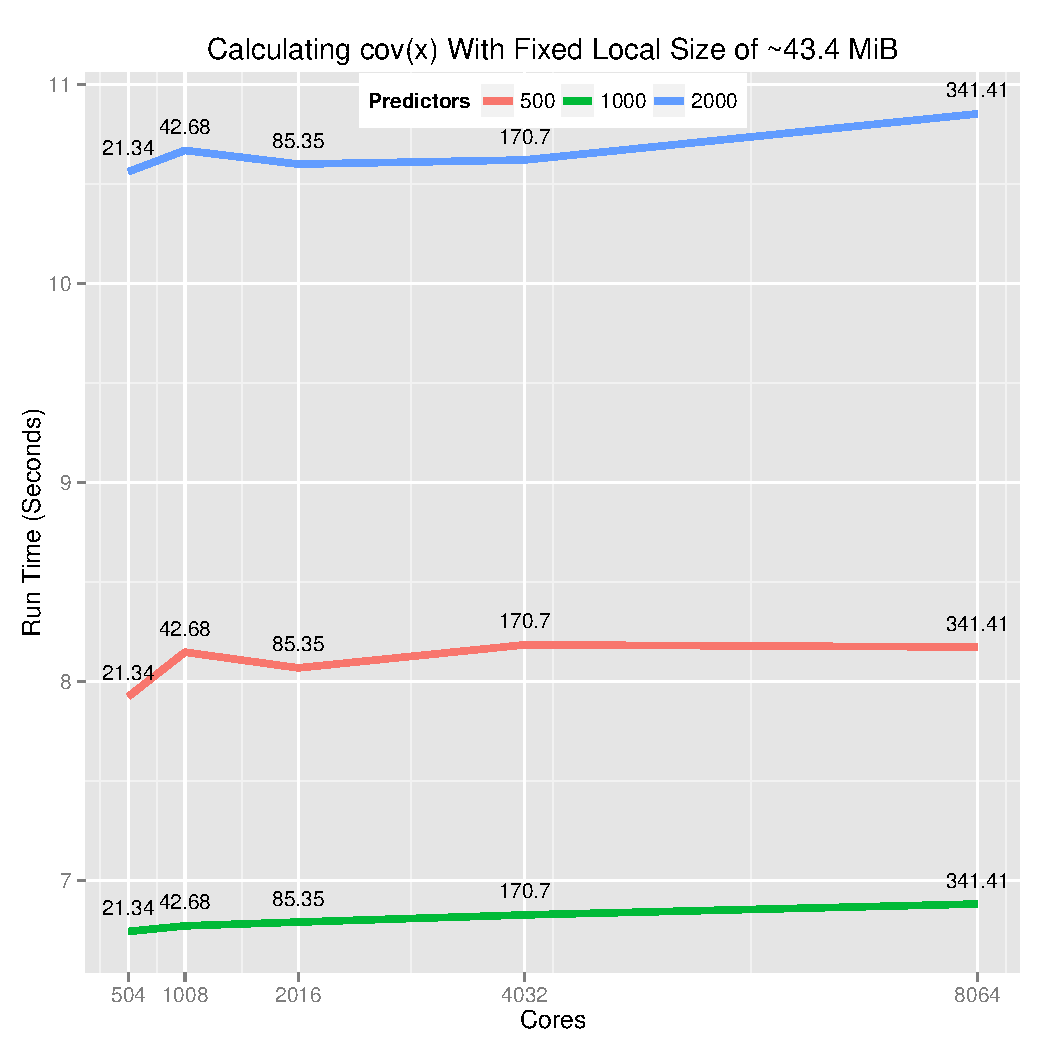
\includegraphics[height=.88\textheight]{../common/pics/cov}
  \end{center}
  \end{block}
\end{frame}

\begin{frame}[fragile]
  \begin{block}{Linear Model Code}
      Find $\bbeta$ such that
      \begin{align*}
      \by = \bX\bbeta + \bepsilon
      \end{align*}

      When $\bX$ is full rank,
      \begin{align*}
      \hat{\bbeta} = (\bX^T\bX)^{-1}\bX^T\by \label{math:ols}
      \end{align*}
\begin{lstlisting}
x <- ddmatrix("rnorm", nrow=n, ncol=p, mean=100, sd=10000)
beta_true <- ddmatrix("runif", nrow=p, ncol=1)

y <- x %*% beta_true

beta_est <- lm.fit(x, y)$coefficients
\end{lstlisting}  %$end
  \end{block}
\end{frame}

\begin{frame}
  \begin{block}{\code{lm.fit()}}
  \begin{center}
    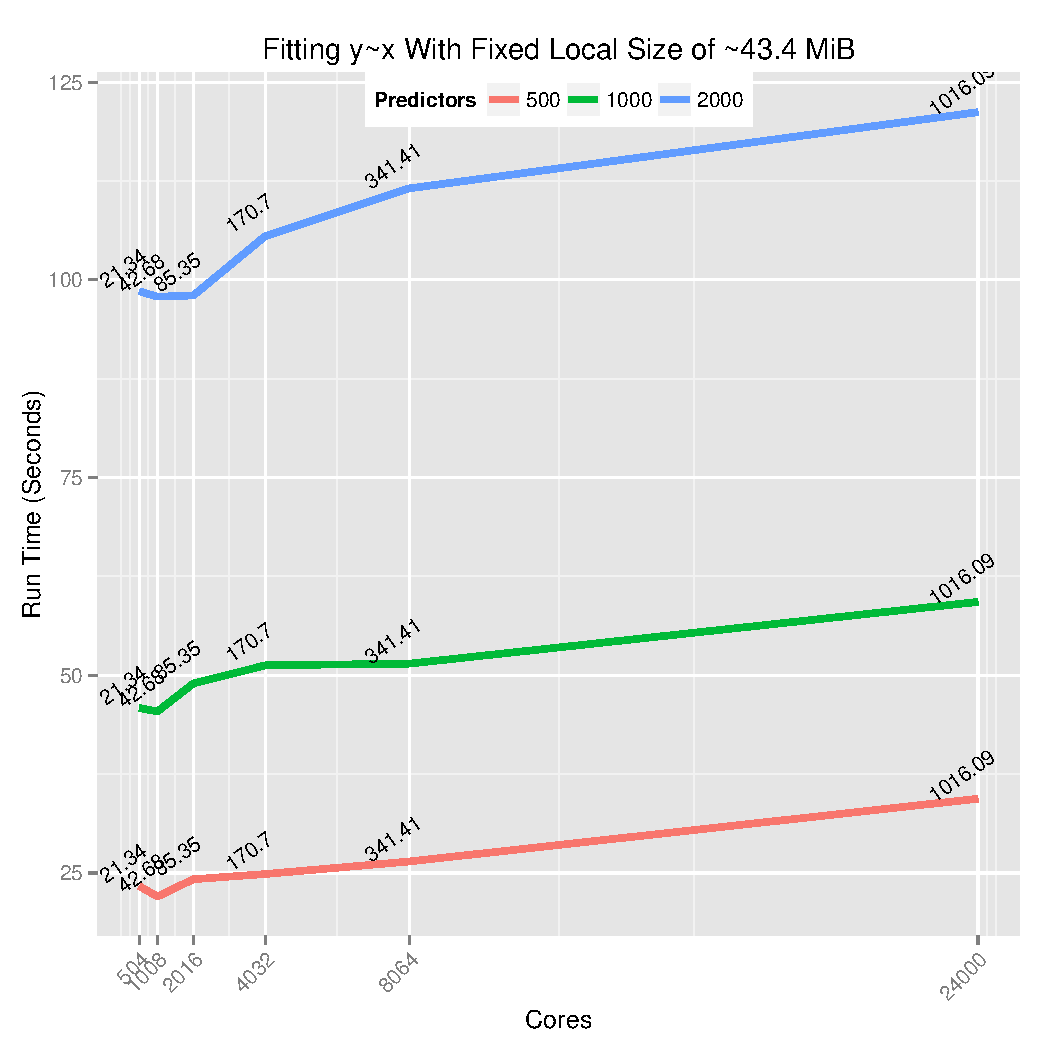
\includegraphics[height=.88\textheight]{../common/pics/benchmarks/lmfit2}
  \end{center}
  \end{block}
\end{frame}

\begin{frame}
  \begin{block}{\code{Data Generation}}
  \begin{center}
    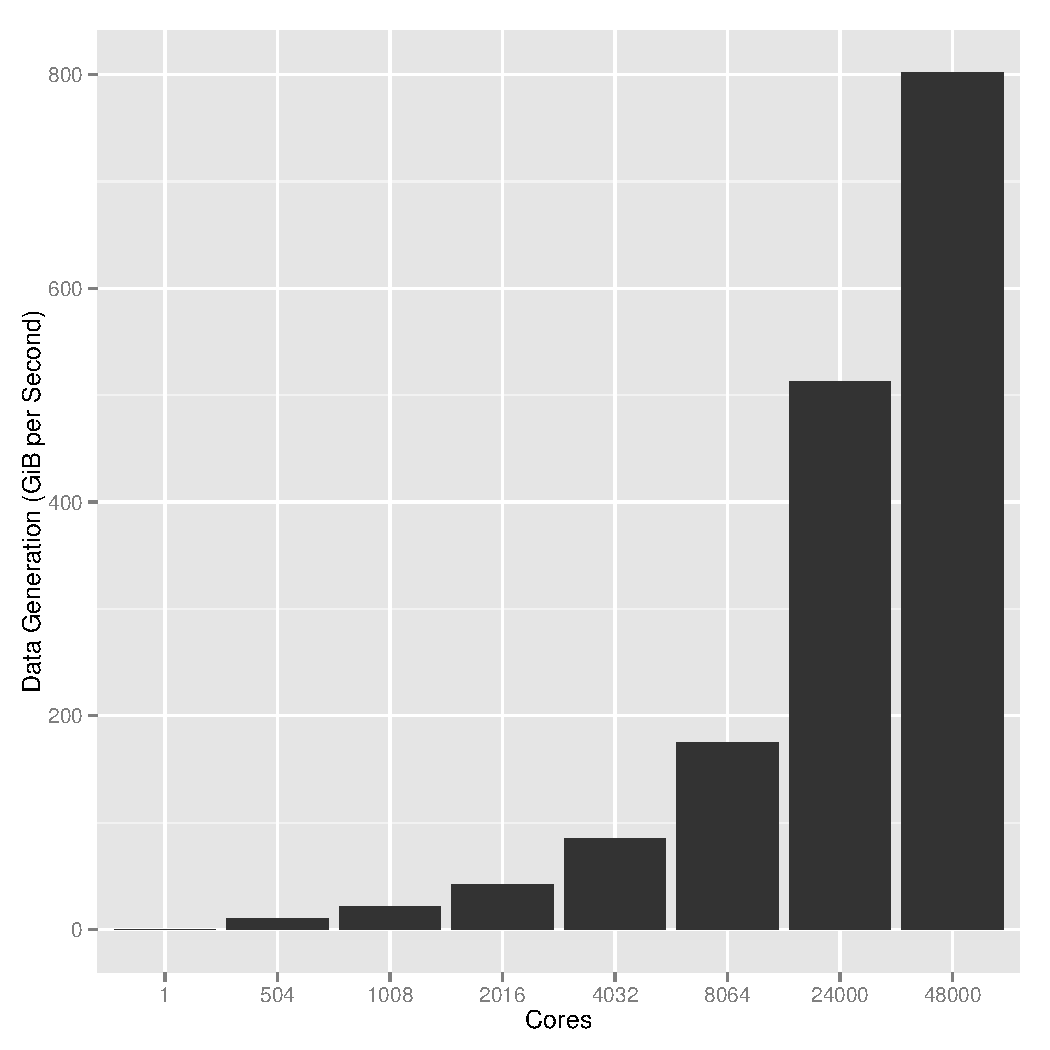
\includegraphics[height=.88\textheight]{../common/pics/benchmarks/datagen24k}
  \end{center}
  \end{block}
\end{frame}

\begin{frame}
  \begin{block}{PCA Benchmark Data}
    \begin{enumerate}[<+-|alert@+>]
      \item Measure wallclock time for principal components analysis
      \item Random normal $N(100, 10000)$
      \item Global problem size fixed
      \item ``strong scaling'' = local problem decreases with core count
      \item Two sets: 50,000 $\times$ 50,000 and 100,000 $\times$ 100,000
      \item Runs out of local work as core count increases
    \end{enumerate}
    \vspace{.8cm}
    \centering
\includegraphics{../common/pics/krakenWide}
  \end{block}
\end{frame}

\begin{frame}
  \begin{block}{\code{prcomp() Strong Scaling}}
  \begin{center}
    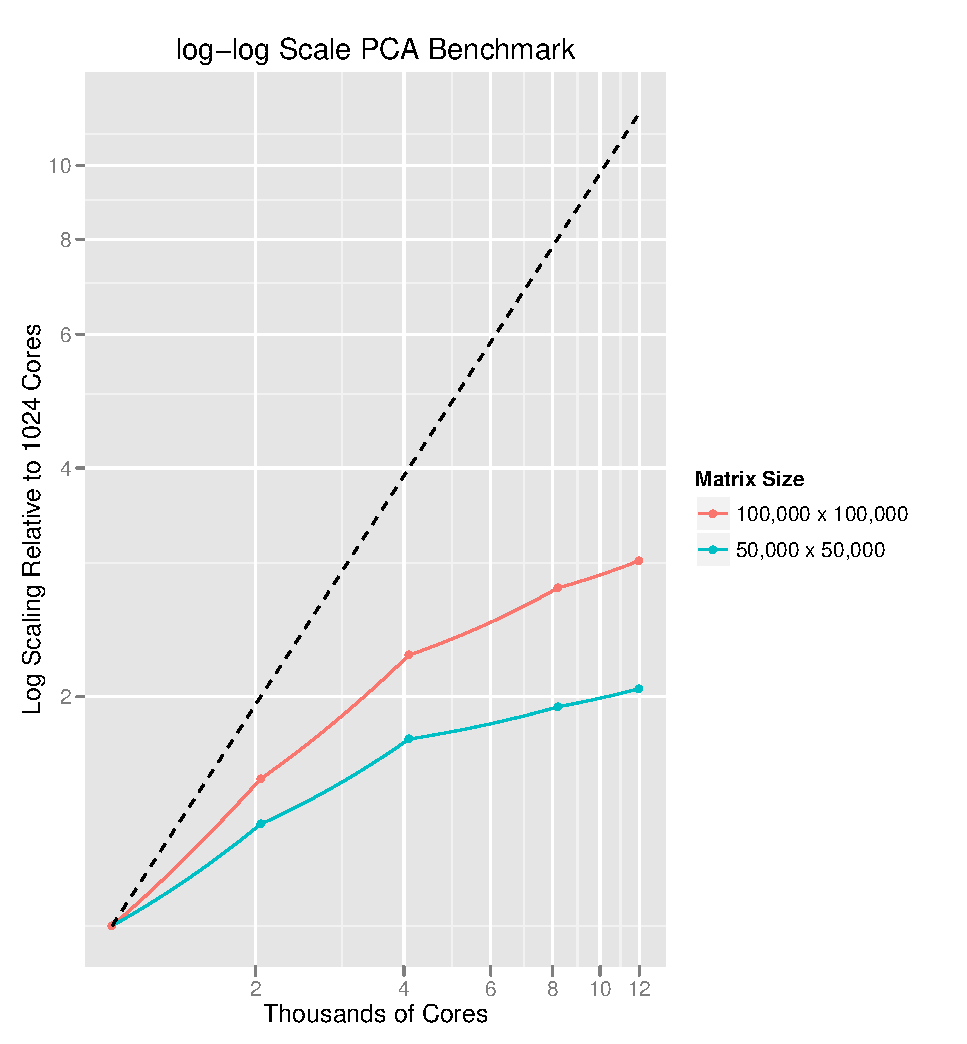
\includegraphics[height=.88\textheight]{../common/pics/benchmarks/pca_scaling}
  \end{center}
  \end{block}
\end{frame}